\section{Process and start/end blocks}
The process block, as the name suggests, is responsible for each action. For programming code analysis, this block corresponds to a function call or an assignment operation. The start / end block in this application differs from the process block only in that it signals the starting point and all possible endings of the algorithm in a given scheme. The application automatically replaces the process blocks at the beginning and end with a start / end block. Additionally, the application ignores all $whitespace$ characters. If we want to enter a space character in the diagram block, use the character "\_" (underscore), which will be replaced. The application does not force the use of syntax elements implying that it is a function call (ending with "... ();") or an assignment (operator "="), to draw this block it is only required that only word characters  are used in any language (if having a Unicode equivalent). 
	
	\begin{figure}[H]
  \begin{subfigure}[t]{0.49\textwidth}
    \vspace{0pt}
    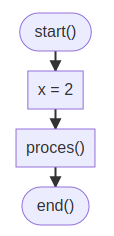
\includegraphics[height=6cm]{proces.png}
  \end{subfigure}\hfill
  \begin{subfigure}[t]{0.49\textwidth}
    \begin{minted}[linenos=true]{cpp}
start();
x _ = _ 2;
proces();
end();
    \end{minted}
  \end{subfigure}%
  \caption{Process, start/end blocks with the code that created those blocks }
\end{figure}

\section{Conditional block }
	\subsection{$if-else$ statement }	 
	
	  The application recognizes the syntax of the statement and creates a decision block from the given condition. Then it creates two branches responsible for actions (any number of process blocks) performed in the event of the condition being met (directly under the scope of the $if$ statement) or not being met (under the scope of the $else$ statement), and then the instructions outside the $if-else$ statement after both branches are being merged.   
		
\begin{figure}[H]
  \begin{subfigure}[t]{0.49\textwidth}
    \vspace{0pt}
    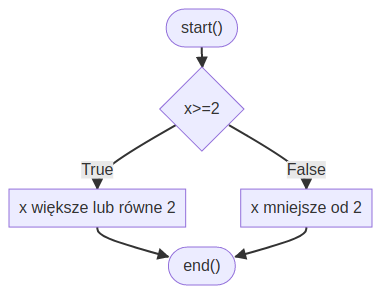
\includegraphics[height=6cm]{decyzja-if.png}
  \end{subfigure}\hfill
  \begin{subfigure}[t]{0.44\textwidth}
    \begin{minted}[xleftmargin=\parindent, linenos=true]{cpp}
start();
if(x >= 2){
  x_większe_lub_równe_2;
}
else{
  x_mniejsze_od_2;
}
end();
    \end{minted}
  \end{subfigure}%
  \caption{Conditional block created with the $if$ statement}
\end{figure}

		\subsection { $while$ statement } 
	
		Interpretacja warunku działa analogicznie jak przy instrukcji $if$, podobnie również działa dołączanie kolejnych instrukcji wykonujących się po spełnieniu warunku z tą różnicą, że ostatni proces tej gałęzi łączony jest automatycznie z bloczkiem decyzyjnym instrukcji $while$. Nie spełnienie warunku odpowiada gałęzi na której znajdują się procesy umieszczone poza scope'm  tego typu instrukcji warunkowej.
	
				\begin{figure}[H]
  \begin{subfigure}[t]{0.49\textwidth}
    \vspace{0pt}
    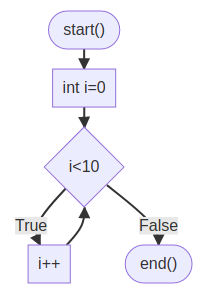
\includegraphics[height=6cm]{decyzja-while.png}
  \end{subfigure}\hfill
  \begin{subfigure}[t]{0.44\textwidth}
    \begin{minted}[linenos=true]{cpp}
start();
int_ i = 0;
while(i < 10){
  i++;
}
end();
    \end{minted}
  \end{subfigure}%
  \caption{Bloczek warunkowy utworzony przy użyciu instrukcji $while$}
\end{figure}	

\section{Bardziej złożony przykład}
Schemat blokowy przedstawiający (uproszczony) algorytm działania aplikacji w której został narysowany: {\smallskip}

			\begin{figure}[H]
  \begin{subfigure}{\textwidth}
    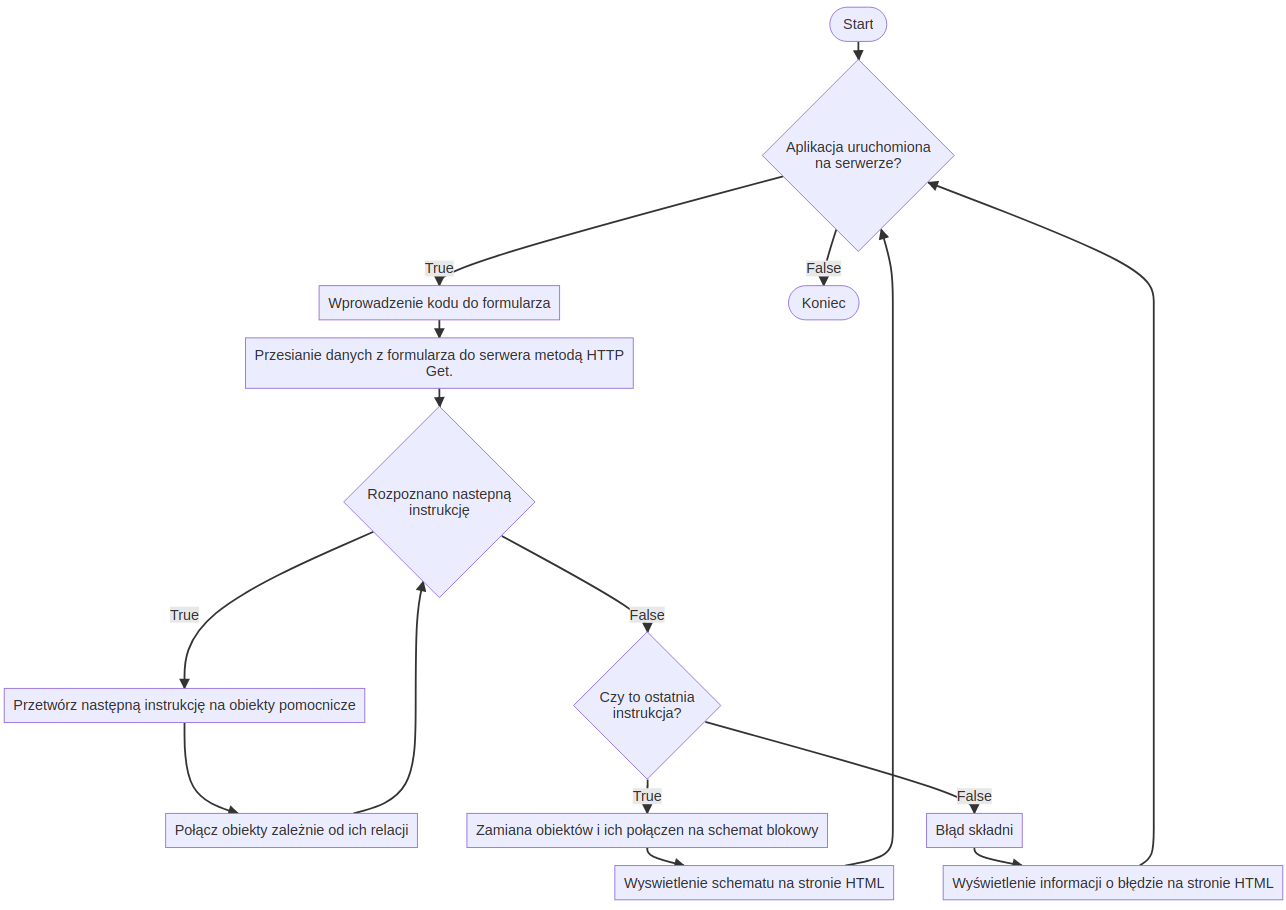
\includegraphics[width=\textwidth]{aplikacja-flowchart.png}
  \end{subfigure}\hfill
  \begin{subfigure}[t]{0.44\textwidth}
    \begin{minted}[linenos=true]{cpp}
Start;
while(Aplikacja _ uruchomiona _ na _ serwerze?){
    Wprowadzenie_ kodu_ do_ formularza;
    Przesianie_ danych_ z_ formularza_ do_ serwera_ metodą_ HTTP_ Get.;
    while(Rozpoznano_ nastepną_ instrukcję){
        Przetwórz_ następną_ instrukcję_ na_ obiekty_ pomocnicze;
        Połącz_ obiekty_ zależnie_ od_ ich_ relacji;
    }
    if(Czy_ to_ ostatnia_ instrukcja?){
    Zamiana_ obiektów_ i_ ich_ połączeń_ na_ schemat_ blokowy;
    Wyswietlenie _ schematu _ na _ stronie _ HTML;
    } else {
        Błąd _ składni;
        Wyświetlenie _ informacji _ o _ błędzie _ na _ stronie _ HTML;
    }
}
Koniec;
    \end{minted}
  \end{subfigure}%
  \caption{Przykład pokazujący obsługę zagnieżdżonych instrukcji warunkowych, zawijanie tekstu oraz wprowadzanie polskich znaków}
\end{figure}